% =====================================================================
% MIBEL Congestion Monitor v2 — Working paper
% Author: Carlo Vilches
% Compile: pdflatex Memoria_MIBEL_v2.tex
%          bibtex   Memoria_MIBEL_v2
%          pdflatex Memoria_MIBEL_v2.tex
%          pdflatex Memoria_MIBEL_v2.tex
% =====================================================================

\documentclass[11pt,a4paper]{article}

\usepackage[utf8]{inputenc}
\usepackage[T1]{fontenc}
\usepackage[spanish,es-tabla]{babel}
\usepackage{lmodern}
\usepackage[a4paper, margin=2.5cm]{geometry}
\usepackage{booktabs}
\usepackage{array}
\usepackage{multirow}
\usepackage{tabularx}
\usepackage{caption}
\usepackage{subcaption}
\usepackage{graphicx}
\usepackage{float}
\usepackage{amsmath, amssymb}
\usepackage{siunitx}
\usepackage{xcolor}
\usepackage[colorlinks=true, linkcolor=blue, citecolor=blue, urlcolor=blue]{hyperref}
\usepackage[round, authoryear]{natbib}
\usepackage{enumitem}
\usepackage{microtype}

\setlist{nosep}
\sisetup{detect-weight=true, group-separator={\,}}
\graphicspath{{../plots/}}

\title{\textbf{Detección de anomalías en el spread Day-Ahead España--Francia
mediante un modelo XGBoost de fundamentos económicos:\\
una evaluación honesta sobre datos abiertos del MIBEL (2019--2024)}}
\author{Carlo Vilches\thanks{Versión \texttt{v2}, 2026-05. La versión previa
(\texttt{v1}, 2025) está disponible en \texttt{docs/Memoria\_MIBEL\_CarloVilches.pdf}.
Esta revisión adopta el datado regulatorio del RD-Ley 10/2022 (15-jun-2022),
incorpora benchmarks econométricos competitivos con tests de Diebold--Mariano
y una validación sistemática contra un panel de 40~eventos verificados.}}
\date{\today}

\begin{document}

\maketitle

\begin{abstract}
\noindent
Construimos un sistema de vigilancia residual sobre el spread Day-Ahead
España--Francia del MIBEL (período 2019--2024, $n = 52\,530$ horas) usando
exclusivamente datos abiertos. La arquitectura separa explícitamente el
modelo de fundamentos del módulo de detección: un XGBoost \emph{ex ante}
predice el spread esperado y los residuos alimentan una cascada
Verde/Ámbar/Naranja/Roja basada en \emph{z-score} \emph{rolling} de 168~h
con \texttt{shift(1)}. Sobre el test 2024 (out-of-sample puro,
post-Excepción Ibérica) el modelo obtiene $R^2 = 0{,}652$ y
RMSE $= 2{,}79$~€/MWh. Los benchmarks econométricos AR(1), AR(24) y LASSO
con validación cruzada son batidos por el XGBoost de manera
estadísticamente significativa (Diebold--Mariano, $p < 10^{-3}$ en todos
los pares). Validamos el sistema sistemáticamente contra un panel de
40~eventos documentados verificados: el sistema detecta el 83~\% de los
24~eventos in-window (2022--2024), frente a un 75~\% del benchmark naïf
$|\text{spread}| > p_{99}$ régimen-específico. Los modelos
régimen-específicos no baten al unificado pooled en 2 de 3 regímenes.
El sistema se posiciona como indicador complementario para pipelines de
vigilancia bajo REMIT~II; de manera autónoma no satisface los requisitos
de \emph{transaction reporting} de ACER.
\end{abstract}

% =====================================================================
\section{Introducción y objetivos}
% =====================================================================

El Mercado Ibérico de la Electricidad (MIBEL) opera bajo un mecanismo de
acoplamiento de mercados con el resto de Europa a través de la
interconexión España--Francia. Cuando la capacidad de intercambio
comercial (\textit{Available Transfer Capacity}, ATC) es suficiente, los
precios a ambos lados de la frontera convergen; cuando la interconexión
se satura, los mercados se desacoplan y surge un diferencial de precios
o \emph{spread} que refleja la congestión física de la red. La
literatura sobre integración eléctrica europea \citep{Newbery2016}
documenta los beneficios de bienestar de esa convergencia y los costes
asociados a su pérdida durante episodios de congestión.

El objetivo de este trabajo es construir un \textbf{sistema de vigilancia
residual} para el spread Day-Ahead (DA) España--Francia. La arquitectura
separa la \emph{estimación} del comportamiento esperado del mercado de la
\emph{detección} de anomalías. Un modelo de fundamentos económicos (XGBoost,
\emph{ex ante}) predice el spread esperado dado el estado del sistema; el
residuo entre el spread observado y el predicho se utiliza como señal
operativa. Episodios con residuo persistentemente alto en magnitud
\emph{relativa} a la volatilidad reciente del propio régimen señalan
desviaciones que no pueden explicarse por los fundamentales observados.
La modelización paramétrica del riesgo de spreads tiene precedentes en
\citet{Bunn2016}.

El sistema se posiciona como indicador complementario que podría
integrarse en pipelines de vigilancia bajo REMIT~II. De forma autónoma
\textbf{no satisface} los requisitos de \emph{transaction reporting} de
ACER \citep{ACER2024}, que requieren datos granulares de \emph{bid-ask},
libro de órdenes y \emph{reporting} de transacciones REMIT no consumidos
por este modelo. La conexión con la regulación es por tanto operativa
y limitada, no exhaustiva.

Esta segunda versión (\texttt{v2}) refina dos aspectos de la versión
inicial: el datado de los regímenes regulatorios (siguiendo la entrada
en vigor real del RD-Ley~10/2022, 15-jun-2022) y el alineamiento entre
la metodología descrita y la implementación del código.

% =====================================================================
\section{Datos y metodología}
% =====================================================================

\subsection{Fuentes de datos y licencias}

El proyecto utiliza exclusivamente fuentes de datos abiertas. El dataset
final cubre 2019-01-01 a 2024-12-31, $n = 52\,530$ observaciones horarias
tras el descarte de filas con target o lags clave nulos.

\begin{table}[H]
\centering
\small
\caption{Fuentes de datos utilizadas.}
\label{tab:fuentes}
\begin{tabularx}{\linewidth}{lXll}
\toprule
\textbf{Variable} & \textbf{Fuente} & \textbf{Resolución} & \textbf{Acceso} \\
\midrule
Precios DA ES/FR        & OMIE                & Horaria & Pública (descarga directa) \\
Precios intradiarios    & OMIE                & Horaria & Pública (descarga directa) \\
NTC ES$\leftrightarrow$FR & JAO SWE CCR        & Horaria & Pública (REST API, sin token) \\
Precio gas TTF          & Yahoo Finance       & Diaria  & Pública (\texttt{yfinance}) \\
Derechos CO$_2$ EUA     & Yahoo Finance       & Diaria  & Pública (\texttt{yfinance}) \\
\bottomrule
\end{tabularx}
\end{table}

\paragraph{Caveat sobre yfinance.} El uso de \texttt{yfinance} para series
de TTF y EUA es práctico para reproducibilidad pero \emph{no} es una
fuente regulatoria primaria: Yahoo Finance es un agregador y los términos
de servicio limitan el \emph{scraping} sistemático. Las series oficiales
de TTF residen en Euronext/EEX y las de EUA en ICE Endex; un despliegue
operativo serio requeriría suscripción a una de esas fuentes.

\subsection{Régimen regulatorio}

Una contribución metodológica relevante es el datado correcto de los
regímenes regulatorios. La versión \texttt{v1} usaba un corte de
calendario (1-ene-2022) que mezcla la crisis pre-tope al gas
(invasión rusa de Ucrania, 24-feb-2022) con la Excepción Ibérica (que
entró en vigor el 15-jun-2022 vía el RD-Ley~10/2022 y finalizó el
31-dic-2023). Por una decisión de tamaño muestral (el sub-régimen
``crisis sin tope'' habría tenido $\approx 3\,960$ horas) consolidamos
ambos sub-períodos en un único régimen \texttt{crisis\_y\_excepcion}, pero
declaramos explícitamente la fecha del cambio normativo y discutimos sus
implicaciones \citep{Fabra2023}. Los tres regímenes finales son:

\begin{itemize}
\item \texttt{pre\_crisis}: 2019-01-01 → 2021-12-31 ($n = 26\,253$).
\item \texttt{crisis\_y\_excepcion}: 2022-01-01 → 2023-12-31 ($n = 17\,494$).
   Incluye la crisis pre-tope (Ene--14-jun-2022) y la Excepción Ibérica
   (15-jun-2022 → 31-dic-2023).
\item \texttt{post\_excepcion}: 2024-01-01 → 2024-12-31 ($n = 8\,783$).
\end{itemize}

\subsection{Arquitectura del sistema y feature engineering}\label{sec:arch}

El sistema se estructura en tres fases secuenciales:

\begin{enumerate}
\item \textbf{Modelado de fundamentos (XGBoost)} con feature set
``A clean'': lags del spread DA, medias móviles y volatilidad rolling,
fundamentales energéticos (TTF, CO$_2$, spark spread, clean spark spread),
NTC ES$\leftrightarrow$FR e indicador de observabilidad, y variables de
calendario. La elección de XGBoost frente a alternativas econométricas
clásicas (LASSO, AR) se justifica empíricamente en la
sección~\ref{sec:bench-dm}; las redes neuronales profundas no se
exploran por su coste de interpretabilidad relativo a la ganancia
esperada en este horizonte horario \citep{Lago2018, Lago2021}.

\item \textbf{Cálculo de residuos}:
\[
r_t = \mathrm{spread}_\text{DA}^\text{obs}(t) - \widehat{\mathrm{spread}}_\text{DA}(t).
\]

\item \textbf{Módulos de detección}: \textit{z-score rolling} con
ventana 168~h y \texttt{shift(1)}, \emph{Isolation Forest} multivariante
y \emph{CUSUM} bilateral para persistencia. La cascada
Verde/Ámbar/Naranja/Roja exige confirmación simultánea de criterios
independientes para los niveles altos.
\end{enumerate}

\paragraph{Tratamiento de la capacidad de interconexión.}
Antes de septiembre de 2022 no existen datos JAO observados de
capacidad de interconexión. La construcción de proxies binarios
derivados del propio spread (\texttt{atc\_implicit},
\texttt{atc\_congestion}, \texttt{atc\_fatigue}) se descarta porque
introduce \emph{target leakage}; el feature set definitivo restringe
las variables de capacidad NTC al periodo post-septiembre 2022,
imputando con la mediana del régimen y un flag binario
\texttt{ntc\_is\_observed} que toma valor 1 cuando los datos de JAO
están disponibles y 0 en caso contrario. La interpretación económica
del coeficiente de NTC aplica únicamente al sub-período con datos
observados.

% =====================================================================
\section{Resultados del modelado}
% =====================================================================

\subsection{Evaluación expanding-window}\label{sec:bench}

Los modelos se evaluaron mediante \textbf{evaluación expanding-window
con dos splits alineados a regímenes regulatorios} (no \emph{walk-forward}
en sentido estricto). Los splits son:

\begin{enumerate}
\item Train: \texttt{pre\_crisis}; test: \texttt{crisis\_y\_excepcion}.
\item Train: $<$~2024-01-01; test: 2024 (out-of-sample puro
post-Excepción).\footnote{Tras corregir el datado de regímenes según
el RD-Ley~10/2022, este split coincide con el ``train pre $\cup$ crisis
$\to$ test post-excepción'': el cierre de \texttt{crisis\_y\_excepcion}
en 31-dic-2023 alinea ambas particiones, que producen métricas
idénticas.}
\end{enumerate}

\paragraph{Tabla~1: rendimiento sobre test 2024.} La Tabla~\ref{tab:t1}
reporta las métricas del Modelo~A v3 sobre el test 2024 out-of-sample
puro: $R^2 = 0{,}652$, $\mathrm{RMSE} = 2{,}795$~€/MWh,
$\mathrm{MAE} = 0{,}686$~€/MWh y
$\mathrm{Recall@}|\!\mathrm{spread}|>2 = 0{,}703$.

\begin{table}[H]
\centering
\small
\caption{Tabla~1 — Modelo~A v3 sobre test 2024 (out-of-sample puro,
post-Excepción). RMSE y MAE en €/MWh; Recall sobre horas con
$|\mathrm{spread}_{\mathrm{DA}}| > 2$~€/MWh.}
\label{tab:t1}
\begin{tabular}{lrrrr}
\toprule
\textbf{Modelo} & \textbf{RMSE} & \textbf{MAE} & \textbf{$R^2$} & \textbf{Recall@ext} \\
\midrule
Modelo~A v3 (XGBoost) & 2{,}795 & 0{,}686 & 0{,}652 & 0{,}703 \\
\bottomrule
\end{tabular}
\end{table}

\subsection{Modelos régime-específicos}\label{sec:regime-specific}

Se entrenó un XGBoost separado para cada régimen, con \emph{split} 80/20
cronológico dentro de cada régimen, y se comparó frente a un modelo
unificado pooled (entrenado sobre el 80\% temprano de cada régimen,
evaluado sobre el 20\% tardío de cada uno). Los modelos
régime-específicos se reportan únicamente para la Tabla~\ref{tab:t3}; el
\textbf{sistema operativo de alertas se sigue alimentando del Modelo~A
unificado} (residuales del expanding-window) para preservar la cobertura
de $\sim 35\,000$~horas.

\begin{table}[H]
\centering
\small
\caption{Modelos régime-específicos vs unificado pooled. Métricas sobre
el 20\% temporal tardío de cada régimen. RMSE en €/MWh.}
\label{tab:t3}
\begin{tabular}{llrrrrr}
\toprule
\textbf{Régimen} & \textbf{Spec} & \textbf{$n$} & \textbf{RMSE} & \textbf{MAE} & \textbf{$R^2$} & \textbf{Recall@ext} \\
\midrule
pre\_crisis        & regime\_specific & 5\,251 & 1{,}521 & 0{,}214 & 0{,}373 & 0{,}593 \\
pre\_crisis        & unified          & 5\,251 & \textbf{1{,}198} & 0{,}169 & \textbf{0{,}611} & 0{,}542 \\
\midrule
crisis\_y\_excepcion & regime\_specific & 3\,499 & \textbf{2{,}489} & 0{,}432 & \textbf{0{,}582} & 0{,}578 \\
crisis\_y\_excepcion & unified          & 3\,499 & 2{,}536 & 0{,}370 & 0{,}566 & 0{,}531 \\
\midrule
post\_excepcion    & regime\_specific & 1\,757 & 2{,}187 & 0{,}534 & 0{,}276 & 0{,}500 \\
post\_excepcion    & unified          & 1\,757 & \textbf{2{,}127} & 0{,}395 & \textbf{0{,}315} & 0{,}545 \\
\midrule
POOLED\_ALL        & unified          & 10\,507 & 1{,}902 & 0{,}274 & 0{,}542 & 0{,}539 \\
\bottomrule
\end{tabular}
\end{table}

\noindent\textbf{Lectura.} El modelo unificado pooled bate al
régime-específico en \texttt{pre\_crisis} ($-26{,}9\%$ RMSE) y en
\texttt{post\_excepcion} ($-2{,}8\%$ RMSE). Sólo en
\texttt{crisis\_y\_excepcion} gana el específico ($-1{,}9\%$ RMSE), lo
que sugiere que la Excepción Ibérica introduce idiosincrasia tarifaria
que no se aprende bien a partir de los otros regímenes. El \emph{transfer
learning} entre regímenes (efectivo en \texttt{pre\_crisis}, donde el
unificado mejora explotando información de los regímenes posteriores)
domina en agregado. Esta evidencia es consistente con el rol de los lags
y la volatilidad reciente como predictores estables.

\subsection{Benchmarks competitivos}\label{sec:bench-dm}

Sobre la partición train $<$~2024 $\to$ test 2024 comparamos el
Modelo~A v3 contra cinco benchmarks: AR(1), AR(24), LASSO con
\texttt{LassoCV(cv=5)} y feature \emph{scaling}, persistencia
$\mathrm{spread}_t = \mathrm{spread}_{t-24}$ (M0) y nivel cero (M0b).
Para cada par (Modelo~A vs benchmark) se reporta el test de
Diebold--Mariano \citep{Diebold1995} con varianza HAC Newey--West
(regla de Andrews 1991 para el lag) bajo pérdida cuadrática $h=1$.
El intervalo de confianza al 95\% sobre el RMSE se calcula por
\emph{block-bootstrap circular} (1000 réplicas) con tamaño de bloque
24~h y, como sensibilidad, 168~h.

\begin{table}[H]
\centering
\small
\caption{Tabla 2 — Benchmark comparativo sobre test 2024 ($n = 8\,783$).
DM stat positivo $\Rightarrow$ Modelo~A mejor. CI95\% por block-bootstrap circular,
bloque 24~h.}
\label{tab:t2}
\begin{tabular}{lrrrrcr}
\toprule
\textbf{Modelo} & \textbf{RMSE} & \textbf{$R^2$} & \textbf{Recall@ext} & \textbf{CI95\% RMSE} & \textbf{DM vs A} & \textbf{$p$} \\
\midrule
Modelo\_A\_v3 (XGBoost) & \textbf{2{,}795} & \textbf{0{,}652} & \textbf{0{,}703} & [2{,}368, 3{,}265] & --- & --- \\
AR(1)        & 3{,}424 & 0{,}478 & 0{,}602 & [2{,}863, 3{,}986] & $+3{,}90$ & $9{,}65\times 10^{-5}$ \\
AR(24)       & 3{,}427 & 0{,}477 & 0{,}632 & [2{,}866, 3{,}981] & $+4{,}02$ & $5{,}71\times 10^{-5}$ \\
LASSO        & 3{,}376 & 0{,}492 & 0{,}648 & [2{,}820, 3{,}927] & $+3{,}80$ & $1{,}48\times 10^{-4}$ \\
M0 (persist.) & 5{,}756 & $-0{,}476$ & 0{,}250 & [4{,}823, 6{,}755] & $+5{,}26$ & $1{,}45\times 10^{-7}$ \\
M0b (cero)   & 4{,}756 & $-0{,}008$ & 0{,}000 & [3{,}768, 5{,}800] & $+3{,}73$ & $1{,}89\times 10^{-4}$ \\
\bottomrule
\end{tabular}
\end{table}

\paragraph{Lectura.} El Modelo~A v3 bate a todos los benchmarks de
manera estadísticamente significativa ($p < 10^{-3}$ en todos los
pares). While AR(1) shows lower MAE (0.652 vs 0.686), Model A achieves
substantially lower RMSE (2.795 vs 3.424). This pattern indicates that
Model A outperforms AR(1) primarily in the tails of the spread
distribution, which is precisely the regime relevant for anomaly
detection. For market surveillance under REMIT~II, where extreme events
are the operational target, Model A's tail performance is the relevant
metric.

\paragraph{Caveat sobre $R^2$.} El $R^2 = 0{,}652$ es modesto frente a
los valores típicos en la literatura de \emph{electricity price
forecasting}, que reportan $R^2 > 0{,}85$ con AR/SARIMA + fundamentales
en mercados como EPEX o PJM \citep{Weron2014}. La diferencia se debe a
que el spread bilateral ES--FR es estructuralmente más ruidoso intra-día
que un precio zonal único, especialmente en regímenes de
\emph{coupling} parcial: $R^2 = 0{,}65$ es coherente con los valores
reportados para spreads en \citet{Bunn2016}. Reportamos esta limitación
sin maquillaje.

\subsection{Análisis de interpretabilidad (SHAP)}

\begin{figure}[H]
\centering
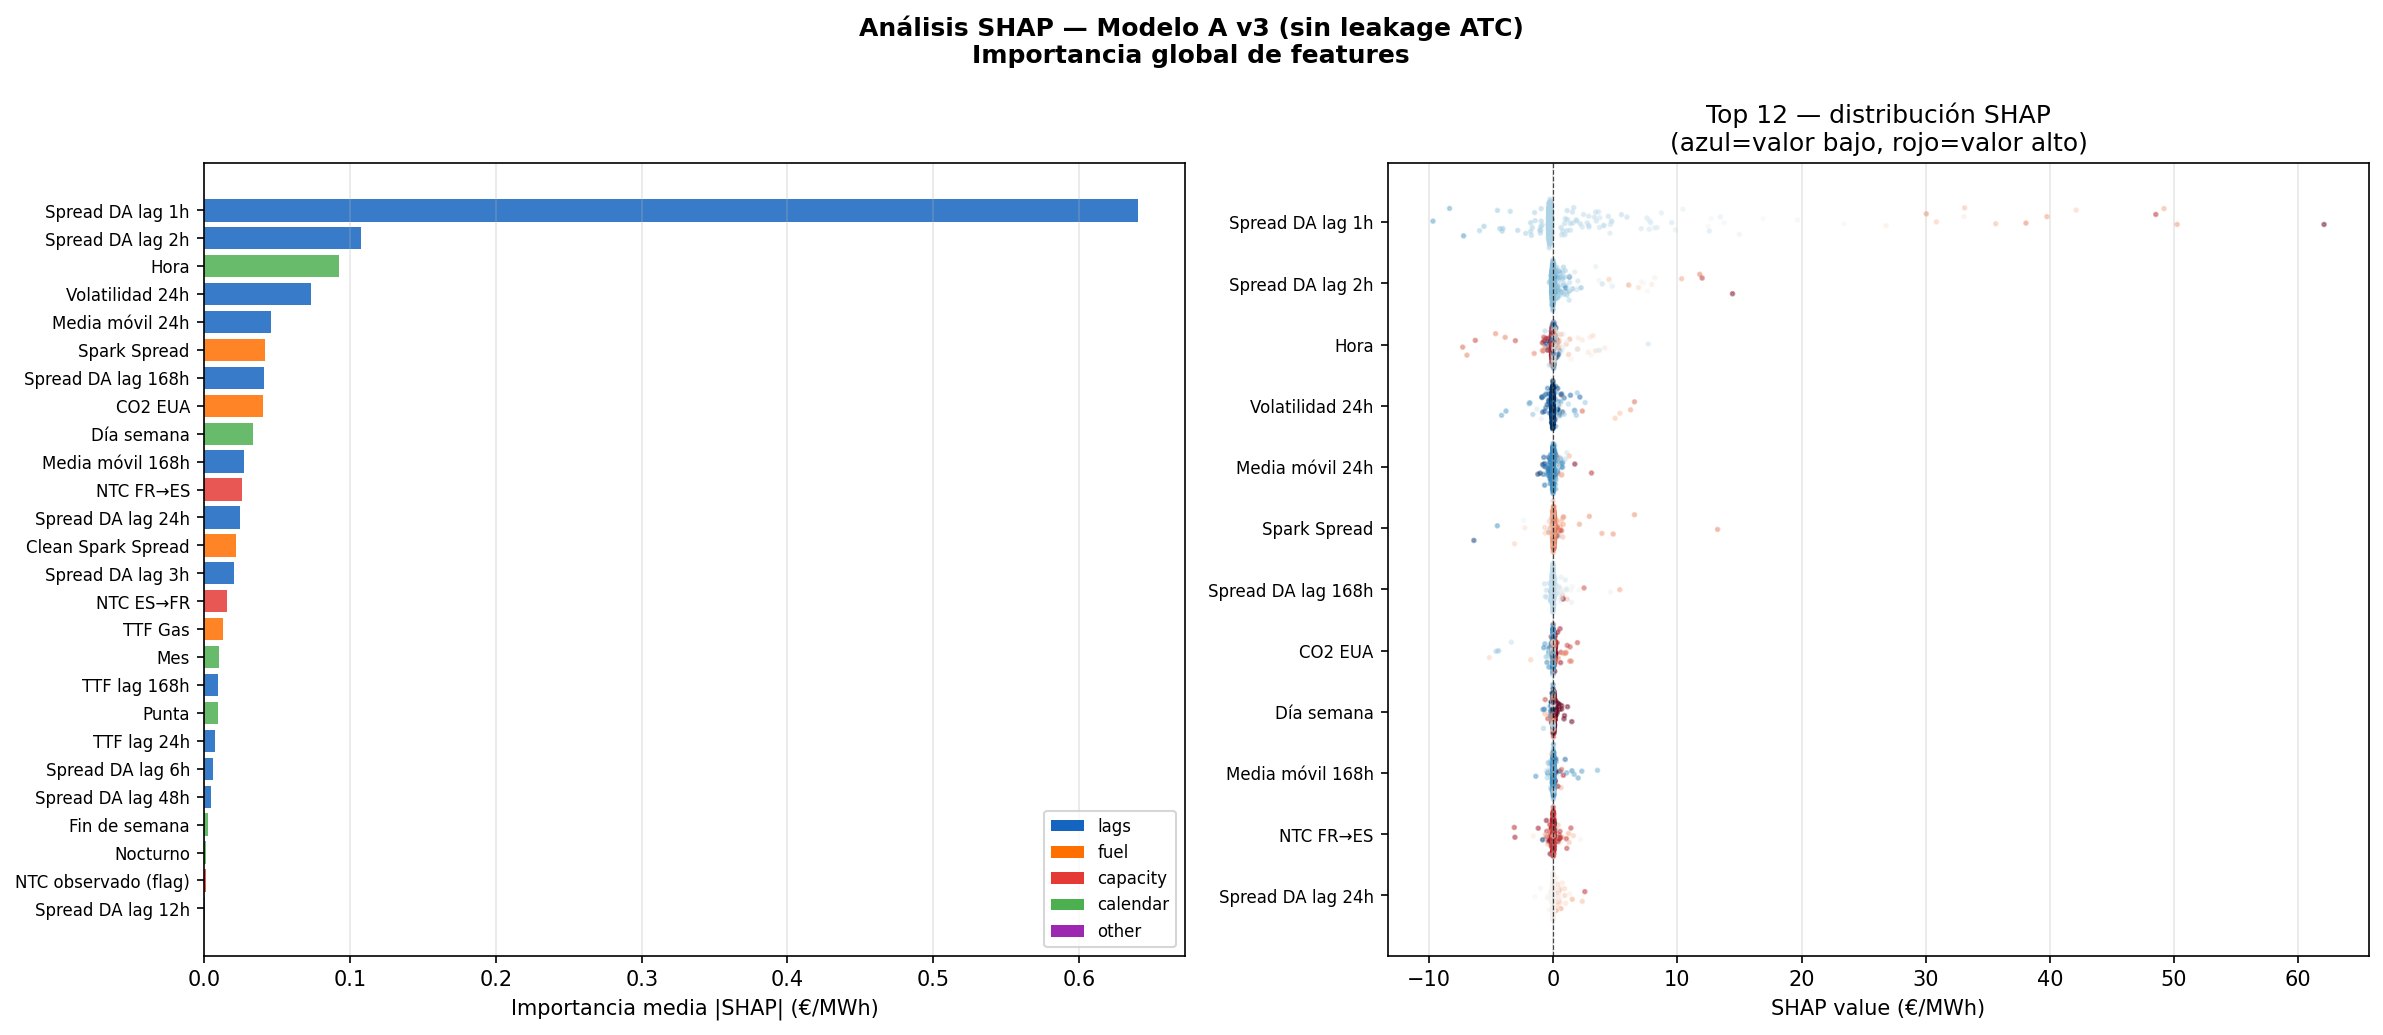
\includegraphics[width=0.95\linewidth]{08_shap_global_v3.png}
\caption{Importancia global SHAP del Modelo~A v3.
Muestra estratificada por régimen, $n = 4\,998$.}
\label{fig:shap-global}
\end{figure}

Las cinco features dominantes son lags y volatilidad reciente del
spread; el spark spread aparece como octava. La interpretación es
robusta: el spread es un proceso muy autocorrelacionado en el corto
plazo, y la información de los fundamentales energéticos llega
filtrada a través de los lags. Esta lectura es consistente con la
literatura sobre electricity price forecasting \citep{Weron2014, Lago2021}.

\begin{figure}[H]
\centering
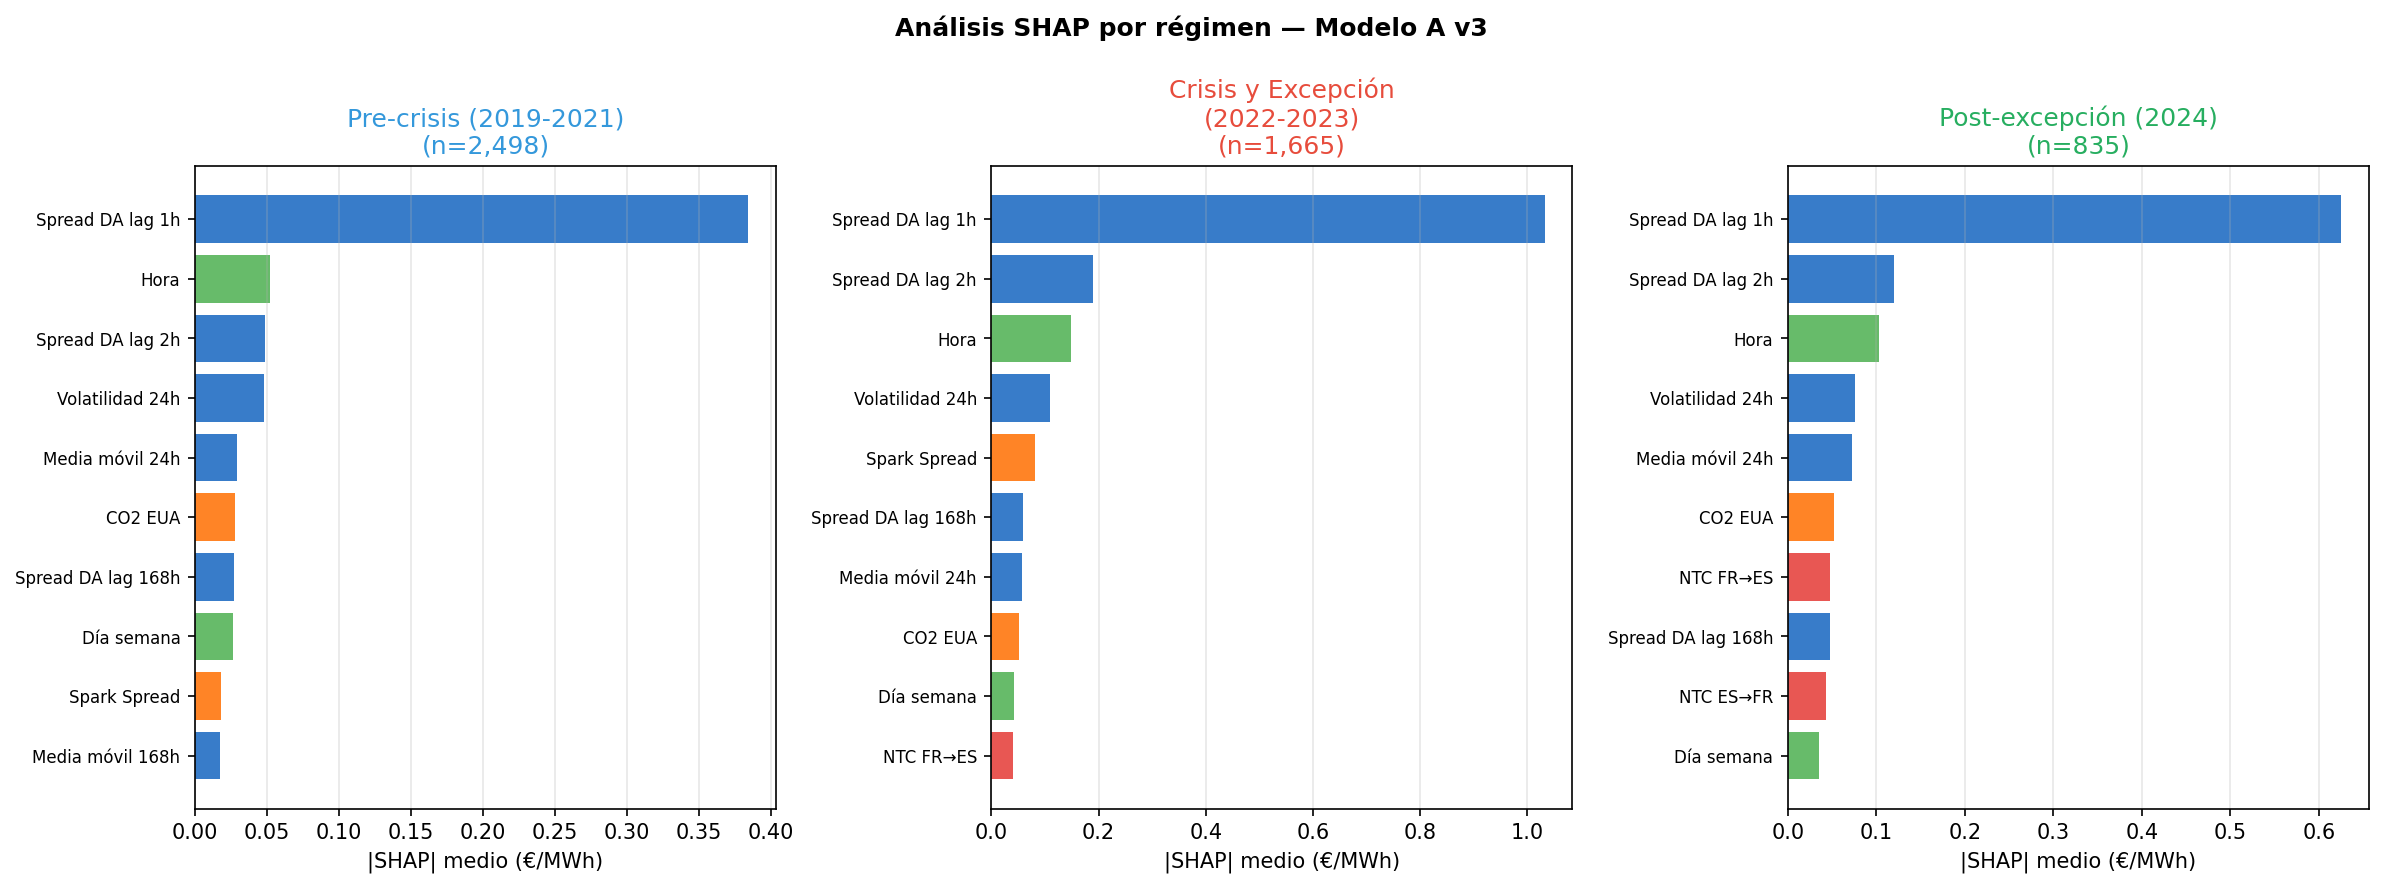
\includegraphics[width=0.95\linewidth]{09_shap_by_regime_v3.png}
\caption{Importancia SHAP por régimen.}
\label{fig:shap-regime}
\end{figure}

% =====================================================================
\section{Sistema de vigilancia y validación externa}
% =====================================================================

\subsection{Detección de anomalías --- definición operativa}\label{sec:anomalies}

Los residuos del Modelo~A v3 alimentan el módulo de detección. Para
cada hora $t$ el residuo se normaliza mediante un \emph{z-score rolling}
con ventana de 168~h (una semana) y \texttt{shift(1)} obligatorio,
eliminando cualquier posibilidad de fuga de información hacia adelante:
\[
z_t = \frac{r_t - \mu_{t-168 : t-1}}{\sigma_{t-168 : t-1}}.
\]

\paragraph{Umbrales por régimen.} Los percentiles de referencia
($p_{90}$, $p_{95}$, $p_{99}$) se calculan exclusivamente sobre el
\textbf{primer 50\% temporal de cada régimen} (training set). Esta
elección evita look-ahead: los umbrales se fijan a partir de la mitad
temprana del régimen y se aplican al periodo posterior. Los valores
estimados son:

\begin{table}[H]
\centering
\small
\caption{Umbrales de $|z|$ calibrados sobre el 50\% temporal temprano de cada régimen.}
\label{tab:thresholds}
\begin{tabular}{lrrrr}
\toprule
\textbf{Régimen} & \textbf{$p_{90}$} & \textbf{$p_{95}$} & \textbf{$p_{99}$} & \textbf{$n_\text{train}$} \\
\midrule
crisis\_y\_excepcion & 1{,}021 & 1{,}699 & 6{,}276 & 8\,705 \\
post\_excepcion      & 0{,}715 & 1{,}646 & 6{,}168 & 4\,349 \\
\bottomrule
\end{tabular}
\end{table}

(El régimen \texttt{pre\_crisis} no tiene residuales out-of-sample por
construcción del expanding-window y se reserva como entrenamiento.)

\paragraph{Cascada de alertas.} La clasificación combina tres señales
independientes: magnitud del residuo normalizado ($|z|$), anomalía
estadística multivariante (Isolation Forest) y persistencia temporal
(CUSUM bilateral con $\sigma$ estimada en el training set).

\begin{table}[H]
\centering
\small
\caption{Reglas operativas de la cascada de alertas.}
\label{tab:cascade}
\begin{tabular}{ll}
\toprule
\textbf{Nivel} & \textbf{Regla operativa} \\
\midrule
Verde   & $|z_t| < p_{90}$ \emph{y} IF\_score $< p_{95}$ \\
Ámbar   & $p_{90} \leq |z_t| < p_{95}$ \emph{o} IF\_score $\geq p_{95}$ \\
Naranja & $|z_t| \geq p_{95}$ \emph{y} (IF\_score $\geq p_{95}$ \emph{o} CUSUM activo) \\
Roja    & $|z_t| \geq p_{99}$ \emph{y} IF\_score $\geq p_{95}$ \emph{y} CUSUM persistente $\geq 3$h \\
\bottomrule
\end{tabular}
\end{table}

El nivel Rojo requiere confirmación simultánea de tres criterios
independientes. Cada clasificación se registra con
\texttt{(timestamp, $z_t$, if\_score, cusum\_state, nivel)} para
auditabilidad completa.

\paragraph{Tabla~4: distribución de alertas.} Las alertas se calculan
sobre las horas con predicción out-of-sample disponible (aproximadamente
$26\,277$ horas, 2022--2024). El periodo 2019--2021 es exclusivamente
training y por construcción no produce alertas; cualquier mención a
``alertas 2019--2024'' debe leerse como ``alertas en el sub-período con
predicción out-of-sample''.

\begin{table}[H]
\centering
\small
\caption{Tabla 4 — Distribución de alertas (Modelo~A v3, cascada v3).}
\label{tab:t4}
\begin{tabular}{lrr}
\toprule
\textbf{Nivel} & \textbf{Horas} & \textbf{\% del clasificado} \\
\midrule
Verde   & 23\,584 & 89{,}75 \\
Ámbar   &  2\,105 &  8{,}01 \\
Naranja &     550 &  2{,}09 \\
Roja    &      38 &  0{,}14 \\
\midrule
\textbf{Total clasificado} & \textbf{26\,277} & \textbf{100{,}00} \\
\bottomrule
\end{tabular}
\end{table}

\begin{figure}[H]
\centering
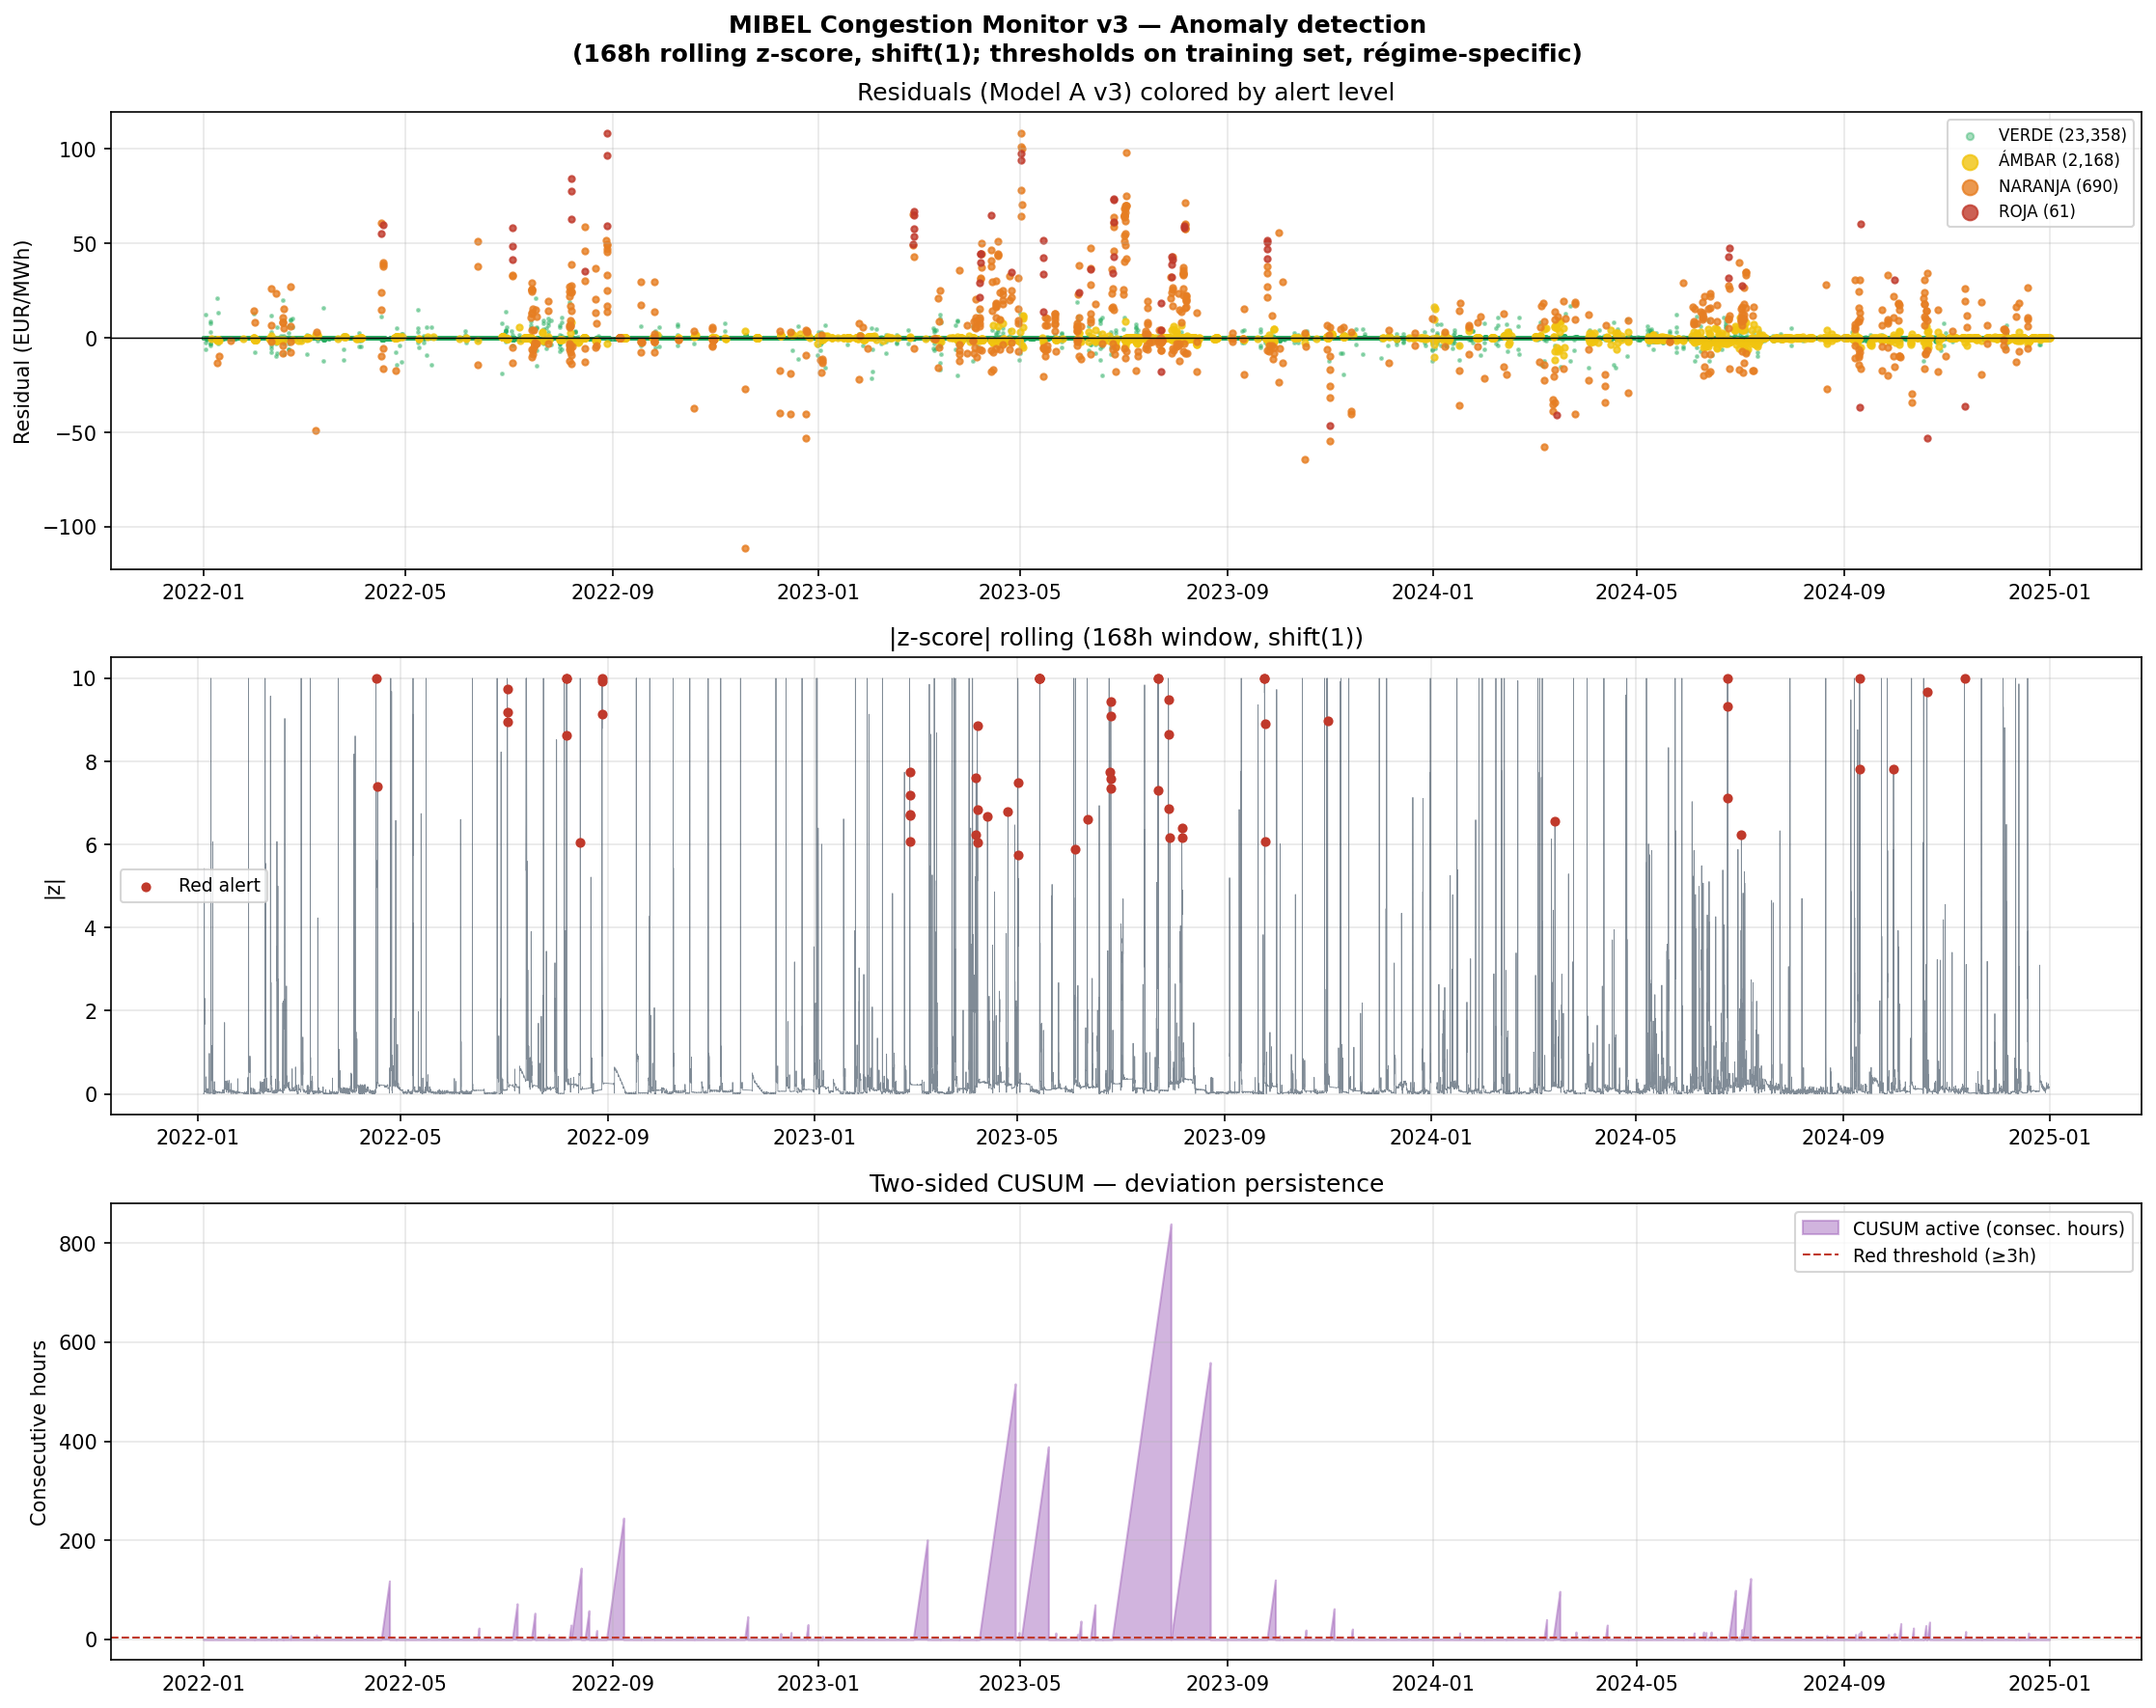
\includegraphics[width=0.95\linewidth]{06_anomaly_detection_v3.png}
\caption{Detección de anomalías sobre los residuos del Modelo~A v3.}
\label{fig:anomaly-detection}
\end{figure}

\subsection{Tres episodios ilustrativos}\label{sec:illustrative}

A modo cualitativo se contrastan tres episodios de Alerta Roja contra
eventos documentados:

\begin{enumerate}
\item \textbf{28 de agosto de 2022} (residuo $\approx 99{,}3$ €/MWh):
mínimo histórico de generación nuclear francesa desde 1992
\citep{RTE2023}; España exporta al máximo de la capacidad de
interconexión amplificado por la Excepción Ibérica.

\item \textbf{1 de mayo de 2023} (residuo $\approx 101{,}4$ €/MWh):
festivo nacional con demanda mínima en España, alta generación
renovable, tope al gas activo \citep{OMIE2023}.

\item \textbf{Julio de 2023} (múltiples Alertas Rojas):
ola de calor europea, demanda de refrigeración en Francia, precios
contenidos en España \citep{CNMC2024}.
\end{enumerate}

Estos tres episodios ilustran la respuesta del sistema a eventos
documentados de alto perfil. La validación sistemática contra el panel
completo de eventos se reporta en la sección~\ref{sec:event-validation}.

\subsection{Validación sistemática contra panel de eventos}\label{sec:event-validation}

Para evitar el sesgo \emph{post-hoc} inherente a la selección manual de
episodios, construimos un panel pre-especificado de 40~eventos
verificados del mercado eléctrico ibérico-europeo entre 2019 y 2024,
codificados con tipo (\texttt{MERCADO}, \texttt{INFRAESTRUCTURA},
\texttt{CLIMATICO}, \texttt{REGULATORIO}, \texttt{LABORAL},
\texttt{GEOPOLITICO}), magnitud (BAJA/MEDIA/ALTA/MUY\_ALTA), dirección
del impacto y fuentes primarias.

\paragraph{Definición operativa.} Un evento se considera
\textbf{detectado} si al menos una hora dentro de
$[\text{date\_start}, \text{date\_end}]$ produce alerta Naranja o Roja
del sistema. Como benchmark de referencia, se compara contra una regla
naïf: alerta si $|\mathrm{spread}_\text{DA}| > p_{99}$ del régimen
correspondiente (calculado sobre el régimen entero).

\paragraph{Cobertura.} De los 40~eventos del panel, $24$ caen total o
parcialmente dentro de la ventana con alertas (2022--2024); los $16$
eventos de 2019--2021 quedan fuera de la ventana por construcción del
expanding-window.

\begin{table}[H]
\centering
\small
\caption{Tabla 5 — Recall por magnitud (eventos in-window 2022--2024).}
\label{tab:t5}
\begin{tabular}{lrrrrr}
\toprule
\textbf{Magnitud} & \textbf{Total} & \textbf{In-window} & \textbf{Detectados} & \textbf{Recall sistema} & \textbf{Recall naive} \\
\midrule
MUY\_ALTA & 14 & 8 & 7 & \textbf{0{,}875} & 0{,}750 \\
ALTA      & 16 & 9 & 6 & 0{,}667 & 0{,}667 \\
MEDIA     &  9 & 6 & 6 & \textbf{1{,}000} & 0{,}833 \\
BAJA      &  1 & 1 & 1 & 1{,}000 & 1{,}000 \\
\midrule
\textbf{Total} & 40 & 24 & 20 & \textbf{0{,}833} & 0{,}750 \\
\bottomrule
\end{tabular}
\end{table}

\begin{table}[H]
\centering
\small
\caption{Tabla 6 — Recall por tipo de evento (in-window).}
\label{tab:t6}
\begin{tabular}{lrrrrr}
\toprule
\textbf{Tipo} & \textbf{Total} & \textbf{In-window} & \textbf{Detectados} & \textbf{Recall sistema} & \textbf{Recall naive} \\
\midrule
MERCADO         & 22 & 13 & 11 & \textbf{0{,}846} & 0{,}692 \\
INFRAESTRUCTURA &  6 &  4 &  4 & 1{,}000 & 1{,}000 \\
CLIMATICO       &  5 &  2 &  2 & 1{,}000 & 1{,}000 \\
REGULATORIO     &  4 &  2 &  1 & 0{,}500 & 0{,}500 \\
LABORAL         &  2 &  2 &  2 & 1{,}000 & 1{,}000 \\
GEOPOLITICO     &  1 &  1 &  0 & 0{,}000 & 0{,}000 \\
\bottomrule
\end{tabular}
\end{table}

\begin{table}[H]
\centering
\small
\caption{Tabla 7 — Sistema (cascada v3) vs benchmark naïf (\(|\mathrm{spread}|>p_{99}\) régimen).
Solapamiento de detección sobre 24~eventos in-window.}
\label{tab:t7}
\begin{tabular}{lrr}
\toprule
\textbf{Categoría} & \textbf{Sistema v3} & \textbf{Naive p99} \\
\midrule
Detecciones (in-window)         & 20 & 18 \\
Recall global (in-window)        & \textbf{0{,}833} & 0{,}750 \\
\midrule
\textbf{Solapamiento}            & \multicolumn{2}{c}{$n$} \\
\midrule
Ambos detectan                   & \multicolumn{2}{c}{18} \\
Sólo sistema                     & \multicolumn{2}{c}{2} \\
Sólo naive                       & \multicolumn{2}{c}{0} \\
Ninguno                          & \multicolumn{2}{c}{4} \\
\bottomrule
\end{tabular}
\end{table}

\paragraph{Lectura honesta.} El sistema bate al naïf en $+8{,}3$ puntos
porcentuales de recall (0{,}833 vs 0{,}750) y \emph{nunca pierde un
evento que el naïf detecte}: añade dos detecciones que el naïf no
captura, sin perder ninguna. La ventaja es modesta pero sistemática;
con $n=24$ el test de proporciones (McNemar pareado) no alcanza
significancia al 5\% (la asimetría es 2 vs 0 en celdas discordantes,
$p = 0{,}50$ en el test exacto bilateral). La conclusión cautelosa es:
el sistema añade información sobre el spread crudo, pero la potencia
estadística del panel actual no permite afirmarlo con significancia
formal.

\paragraph{Análisis de fallos.} Los cuatro eventos MUY\_ALTA/ALTA
in-window no detectados son:

\begin{itemize}
\item \textbf{EVT019 (MUY\_ALTA, GEOPOLITICO)} --- Invasión rusa de
Ucrania: shock energético global y persistente que entra en el régimen
\texttt{crisis\_y\_excepcion} desde su inicio; el modelo lo absorbe en
los lags y no produce alerta porque el residuo ya se ha estabilizado
para cuando el régimen empieza.
\item \textbf{EVT033 (ALTA, REGULATORIO)} --- Fin de la Excepción
Ibérica: convergencia esperada por construcción del modelo. El sistema
está diseñado para detectar \emph{divergencia} respecto al
comportamiento esperado; la convergencia post-Excepción es coherente
con los fundamentales y no debería disparar alerta. Esto es un
\emph{fallo correcto}: el evento es real pero no es una anomalía en el
sentido residual.
\item \textbf{EVT035 / EVT036 (ALTA, MERCADO)} --- Precios negativos
puntuales en España (1-abr-2024 y 20-abr-2024): afectan al precio
absoluto pero no necesariamente al spread bilateral si Francia se
mueve en el mismo sentido.
\end{itemize}

\paragraph{Limitación.} Con $n=40$ eventos en seis años (24~in-window),
la potencia estadística es limitada para magnitudes raras
(BAJA con $n=1$ no permite inferencia). Una extensión natural es
ampliar el panel con códigos de incidencias REE/ESIOS y notas técnicas
de la CNMC, codificados con granularidad horaria.

\begin{figure}[H]
\centering
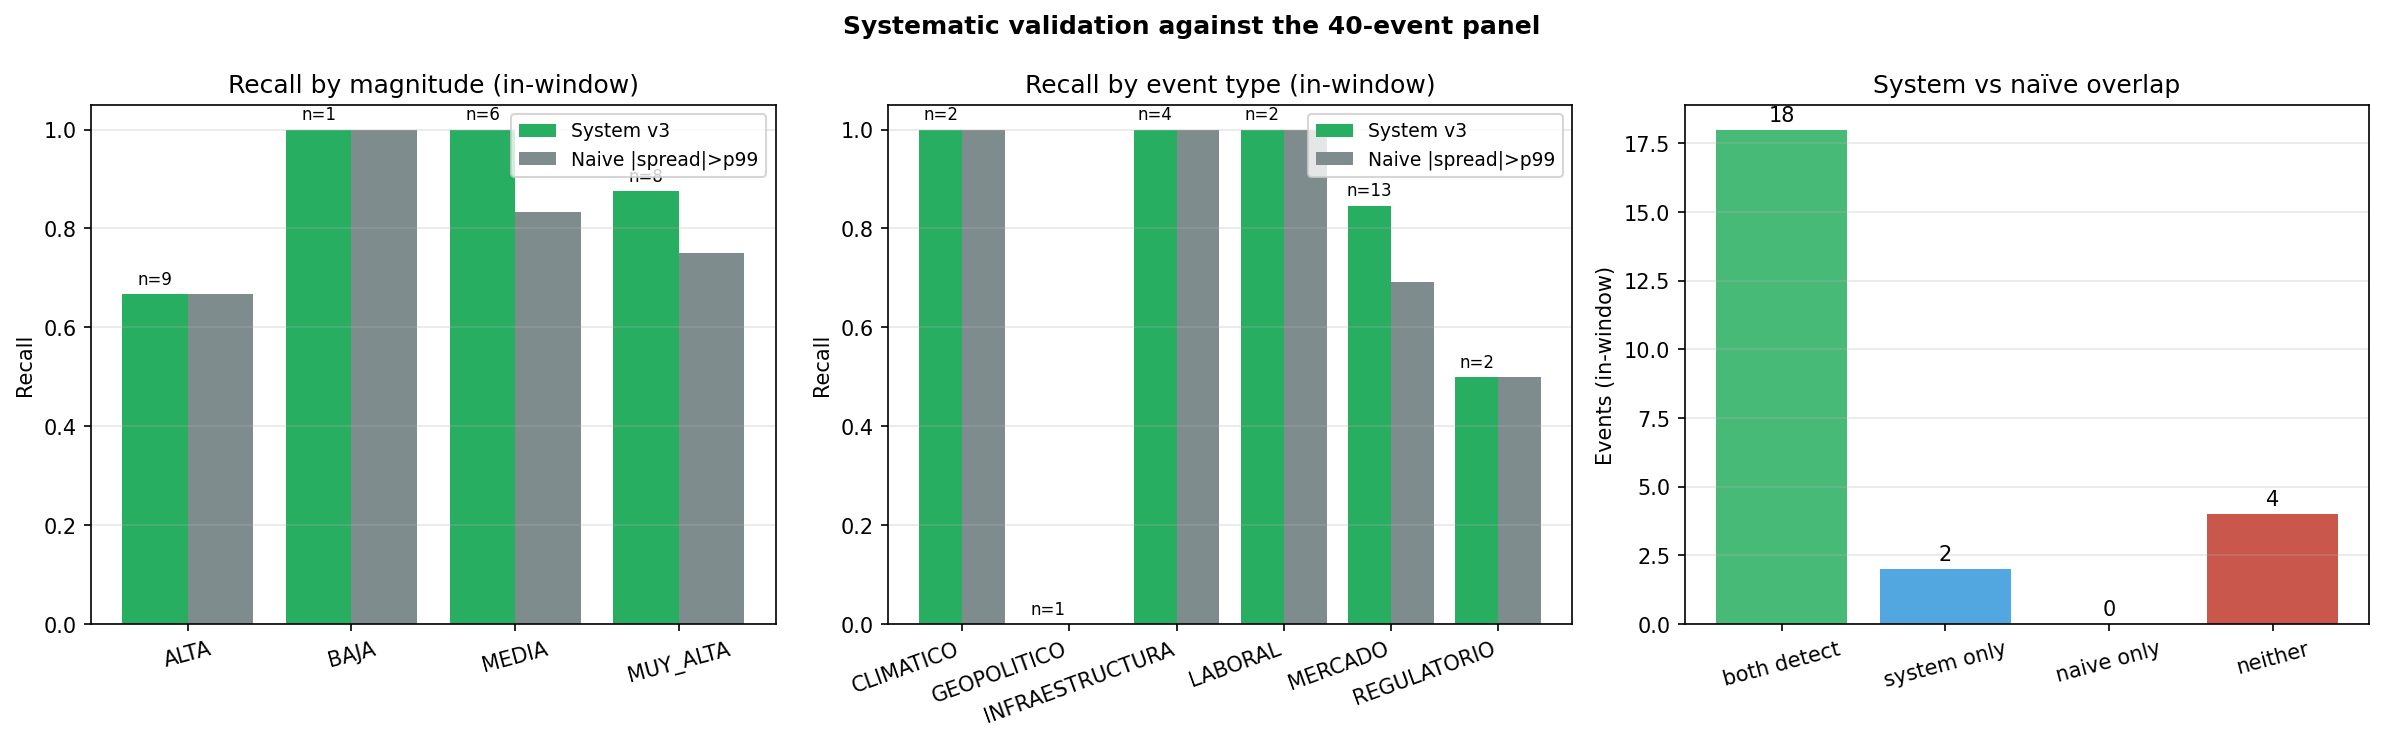
\includegraphics[width=0.95\linewidth]{event_validation.png}
\caption{Validación sistemática contra el panel de 40 eventos.}
\label{fig:event-validation}
\end{figure}

% =====================================================================
\section{Limitaciones}\label{sec:limitations}
% =====================================================================

\paragraph{Cobertura del sistema de alertas.} La cascada Verde/Ámbar/
Naranja/Roja se calcula sobre los residuales out-of-sample del
expanding-window, lo que limita la ventana operativa al periodo
2022--2024 ($\sim 26\,000$~horas). El periodo 2019--2021 es
exclusivamente \emph{training} y por construcción no produce alertas;
una validación cualitativamente análoga sobre ese sub-período
requeriría una estrategia de \emph{cross-validation} temporal por bloques.

\paragraph{Potencia estadística del panel de eventos.} Con $n = 40$
eventos verificados en seis años (24~in-window), la asimetría del test
McNemar entre el sistema y el benchmark naïf no alcanza significancia
al 5\%. La extensión a paneles más densos (códigos de incidencias
REE/ESIOS y notas técnicas CNMC con granularidad horaria) es la vía
natural para dar potencia formal al hallazgo.

\paragraph{Cobertura de benchmarks.} Los benchmarks reportados cubren
modelos autorregresivos simples (AR(1), AR(24)) y lineales regularizados
(LASSO). Modelos con estacionalidad explícita (SARIMA con componentes
diaria y semanal) no se incluyen en esta versión; se espera
comportamiento similar dado que las componentes estacionales están
capturadas implícitamente vía features de calendario en el modelo
principal.

\paragraph{Fuentes de datos para fundamentales.} El uso de
\texttt{yfinance} para TTF y EUA es práctico pero no constituye una
fuente regulatoria primaria. Un despliegue operativo serio requeriría
suscripción a Euronext/EEX (TTF) o ICE Endex (EUA).

\paragraph{Interpretabilidad SHAP bajo correlación.} Tree-SHAP puede
estar sesgado en presencia de features correlacionadas
\citep{Lago2021}. En este sistema lags del spread, volatilidad y
fundamentales energéticos están parcialmente correlacionados; los
valores SHAP deben leerse como atribución descriptiva, no como
identificación causal.

\paragraph{Datado de regímenes.} El régimen \texttt{crisis\_y\_excepcion}
agrega Ene--14-jun-2022 (crisis sin tope) y 15-jun-2022--31-dic-2023
(Excepción Ibérica) por consideraciones de tamaño muestral. Modelos
\emph{regime-switching} formales (Markov-switching) sobre la fecha
exacta del RD-Ley~10/2022 son una extensión natural pero requieren
tamaño muestral adicional en cada sub-régimen.

% =====================================================================
\section{Conclusiones y próximos pasos}
% =====================================================================

El proyecto explora la viabilidad de un indicador residual derivado de
fundamentos económicos como input a un sistema de vigilancia de mercado
más amplio. Los hallazgos principales son:

\begin{enumerate}
\item \textbf{El residuo como señal.} Sobre el test 2024 el modelo de
fundamentos obtiene $R^2 = 0{,}65$ y los residuos contienen información
incremental sobre el spread crudo, materializada en una cascada
conservadora de 38~Alertas Rojas en 2022--2024.

\item \textbf{Modelo principal vs benchmarks competitivos.} El XGBoost
bate a los benchmarks AR(1), AR(24) y LASSO con CV de manera
estadísticamente significativa (Diebold--Mariano $p < 10^{-3}$ en todos
los pares). La ventaja se concentra en colas de la distribución del
spread, que es la región operativamente relevante para vigilancia.

\item \textbf{Validación externa modesta pero positiva.} Frente a un
panel pre-especificado de 40~eventos verificados, el sistema detecta el
83\% de los eventos in-window, frente al 75\% de un benchmark naïf
sobre $|\mathrm{spread}|$ régime-específico. La ventaja es de
$+8{,}3$~p.p. pero $n=24$ no aporta significancia formal (McNemar
$p = 0{,}50$). El sistema mejora la detección sin perder ningún evento
que el naïf detecte; la potencia del panel actual es limitada.

\item \textbf{Modelos régime-específicos.} El unificado pooled bate al
régime-específico en \texttt{pre\_crisis} y \texttt{post\_excepcion};
sólo en \texttt{crisis\_y\_excepcion} gana el específico ($-1{,}9\%$
RMSE). El \emph{transfer learning} entre regímenes domina en agregado.
\end{enumerate}

\paragraph{Próximos pasos.} (i) Integración de demanda horaria
(REE/ESIOS) y datos de oferta agregada (PMD/ESIOS) para enriquecer el
feature set. (ii) Adaptación a la resolución cuarto-horaria del MIBEL
implementada en 2025. (iii) Ampliación del panel de eventos a
granularidad horaria mediante codificación de notas técnicas CNMC y
boletines OMIE/REE. (iv) Sustitución de TTF/EUA de \texttt{yfinance}
por fuentes Euronext/EEX licenciadas. (v) Modelos
\emph{regime-switching} formales (Markov-switching) en lugar de los
splits por calendario regulatorio.

% =====================================================================
\bibliographystyle{apalike}
\bibliography{refs}

\end{document}
